% =============================================================================
% CHAPTER 25: The Complete Optimization Problem
% =============================================================================
% Version: 1.0 (January 2026)
% Type: A (CORE Chapter)
% Purpose: Present the unified optimization problem integrating all 24 chapters
% Primary Appendix: MP (CORE-MASTER)
% Prerequisites: Chapters 1-24, familiarity with 10C framework
% Leads to: Conclusion, Policy Implementation
% =============================================================================

\chapter{The Complete Optimization Problem}
\label{ch:complete-optimization}

% =============================================================================
% METADATA BLOCK
% =============================================================================
\begin{tcolorbox}[colback=gray!5!white,colframe=gray!75!black]
\small
\textbf{Chapter Type:} A (CORE Chapter) \\
\textbf{Version:} 1.0 \\
\textbf{Purpose:} Present the unified optimization problem integrating all 24 chapters \\
\textbf{Primary Appendix:} MP (CORE-MASTER) \\
\textbf{Prerequisites:} Chapters 1--24, 10C Framework \\
\textbf{Leads to:} Conclusion, Policy Implementation
\end{tcolorbox}

% =============================================================================
% QUICK REFERENCE BOX
% =============================================================================
\begin{tcolorbox}[colback=blue!5!white,colframe=blue!75!black,
    title=\textbf{Quick Reference: Key Concepts in This Chapter}]
\small
\begin{tabular}{@{}p{3.5cm}p{9cm}@{}}
\textbf{Master Problem} & $\max \sum_t \delta^t P_{eff}(S_t, I_t, \Psi_t)$ \\[3pt]
\textbf{Objective Function} & $P_{eff} = \sigma(WEC \cdot \alpha_{BCJ} \cdot \beta_{BCS})$ \\[3pt]
\textbf{State Space (10C)} & $S = (L, d, \gamma, \Psi, \Theta, A, W, \varphi, N_{L2})$ \\[3pt]
\textbf{Instruments} & $\vec{I} \in [0,1]^9$ (9D intervention vector) \\[3pt]
\textbf{Constraints} & C1--C7 (Budget, Crowding, Timing, Capacity, Ethics, Segment, K*) \\[3pt]
\textbf{Key Insight} & Landscape has multiple equilibria; optimal portfolio size K* emerges \\
\end{tabular}
\end{tcolorbox}

% =============================================================================
% APPENDIX REFERENCES BOX
% =============================================================================
\begin{tcolorbox}[colback=green!5!white,colframe=green!75!black,
    title=\textbf{Appendix References}]
\small
\textbf{Primary:}
\begin{itemize}[noitemsep]
    \item \textbf{MP (CORE-MASTER):} Complete mathematical formulation, 140 axioms, 62 theorems
\end{itemize}
\textbf{Supporting:}
\begin{itemize}[noitemsep]
    \item \textbf{AAA--HI:} The 10 CORE appendices defining state space components
    \item \textbf{IE (CORE-EIT):} Intervention emergence and 9D vector
    \item \textbf{FRM (LIT-FEHR-METHOD):} Exclusion Principle (EXC-1 to EXC-6)
    \item \textbf{BBB (CORE-WHERE):} Parameter calibration values
\end{itemize}
\end{tcolorbox}

% =============================================================================
% CHAPTER SCOPE BOX
% =============================================================================
\begin{tcolorbox}[colback=orange!5!white,colframe=orange!75!black,
    title=\textbf{Chapter Scope: Ziel / In-Scope / Out-of-Scope / Lieferobjekte}]

\textbf{Ziel (Objective):}
\begin{itemize}[nosep]
    \item Present the complete optimization problem that integrates all 24 chapters
    \item Answer: \textit{How do we maximize sustainable behavioral change over time?}
\end{itemize}

\textbf{In-Scope:}
\begin{itemize}[nosep]
    \item The Master Problem formulation
    \item 10C state space mapping
    \item Constraint system (C1--C7)
    \item Dynamic programming structure (Bellman equation)
    \item Key structural properties (non-concavity, multiple equilibria)
    \item The 4-Stage Pipeline: $U_{pot} \to U_{eff} \to WAX \geq \theta \to S(t)$
\end{itemize}

\textbf{Out-of-Scope (delegiert an Appendix MP):}
\begin{itemize}[nosep]
    \item Full axiom catalog (140 axioms) $\rightarrow$ Appendix MP
    \item Complete theorem proofs (62 theorems) $\rightarrow$ Appendix MP
    \item Solution algorithms $\rightarrow$ Appendix AN (METHOD-LLMMC)
    \item Empirical calibration $\rightarrow$ Appendix BBB (CORE-WHERE)
\end{itemize}

\textbf{Lieferobjekte (Deliverables):}
\begin{itemize}[nosep]
    \item Master Problem equation with intuitive explanation
    \item 10C-to-State mapping table
    \item Chapter contribution matrix
    \item Visual representation of the optimization landscape
\end{itemize}

\end{tcolorbox}

% =============================================================================
% CORE CONNECTION BOX (TYPE A CHAPTER)
% =============================================================================
\begin{tcolorbox}[colback=purple!5!white,colframe=purple!75!black,
    title=\textbf{CORE Connection: MP (CORE-MASTER)}]

This chapter corresponds to \textbf{Appendix MP (CORE-MASTER)}, which provides the complete mathematical formulation of the EBF optimization problem.

\textbf{Relationship:}
\begin{itemize}[noitemsep]
    \item This chapter: Conceptual overview, intuition, accessibility
    \item Appendix MP: Complete formalism, 140 axioms, 62 theorems, full proofs
\end{itemize}

\textbf{10C Integration:} MP integrates ALL 10 CORE dimensions into a unified state space $S$.

\end{tcolorbox}

% =============================================================================
% INTUITION BOX
% =============================================================================
\begin{tcolorbox}[colback=yellow!5!white,colframe=yellow!75!black,
    title=\textbf{Intuition: Anna's Journey to the Complete Picture}]

\textit{Anna, a behavioral economist, has spent months studying the EBF framework. She understands awareness (Chapter 11), willingness (Chapter 12), the behavioral change journey (Chapter 13), and intervention design (Chapters 17-20). But she asks: ``How does it all fit together?''}

\textit{This chapter answers Anna's question. It shows that all 24 chapters contribute to a single optimization problem: maximizing the probability of sustainable behavioral change over time. Each chapter provides one piece of the puzzle---this chapter assembles them into the complete picture.}

\textit{``It's like finally seeing the entire map after studying individual regions,'' Anna realizes. ``The optimization problem IS the framework.''}

\end{tcolorbox}

% =============================================================================
% CENTRAL QUESTION BOX
% =============================================================================
\begin{tcolorbox}[colback=red!5!white,colframe=red!75!black,
    title=\textbf{Central Question}]
\begin{center}
\Large\textit{How do we maximize the probability of sustainable behavioral change over time, given the 10C state, context dynamics, and intervention constraints?}
\end{center}
\end{tcolorbox}

% =============================================================================
% CHAPTER OVERVIEW
% =============================================================================
\section*{Chapter Overview}

This chapter presents the complete optimization problem that unifies the entire EBF framework:

\begin{enumerate}
    \item \textbf{Section~\ref{sec:25-master-problem}:} The Master Problem---the single equation that captures everything
    \item \textbf{Section~\ref{sec:25-state-space}:} The 10C State Space---how each CORE dimension contributes
    \item \textbf{Section~\ref{sec:25-objective}:} The Objective Function---what we're maximizing
    \item \textbf{Section~\ref{sec:25-constraints}:} The Constraint System---C1 to C7
    \item \textbf{Section~\ref{sec:25-dynamics}:} Dynamic Structure---the Bellman equation
    \item \textbf{Section~\ref{sec:25-properties}:} Structural Properties---non-concavity, multiple equilibria
    \item \textbf{Section~\ref{sec:25-pipeline}:} The 4-Stage Pipeline---from potential to sustained change
    \item \textbf{Section~\ref{sec:25-integration}:} Chapter Integration Matrix---what each chapter contributes
    \item \textbf{Section~\ref{sec:25-workflow}:} Practical Workflow---the 7-step process from problem to portfolio
\end{enumerate}


% =============================================================================
% SECTION 1: THE MASTER PROBLEM
% =============================================================================
\section{The Master Problem}
\label{sec:25-master-problem}

\subsection{The Central Equation}
\label{sec:25-central-equation}

The entire EBF framework can be expressed as a single optimization problem:

\begin{tcolorbox}[colback=blue!5!white,colframe=blue!75!black,
    title=\textbf{The EBF Master Problem (MP-1)}]
\begin{equation}
\max_{I_t \in \mathcal{I}} \sum_{t=0}^{T} \delta^t \cdot P_{eff}(S_t, I_t, \Psi_t)
\label{eq:master-problem}
\end{equation}

\textbf{Subject to:}
\begin{align}
    S_{t+1} &= g(S_t, I_t, a_t) & \text{(State transition)} \\
    \Psi_{t+1} &= f(\Psi_t, I_t, a_t) & \text{(Context evolution)} \\
    I_t &\in [0,1]^9 & \text{(Intervention bounds)} \\
    C_1, \ldots, C_7 &\text{ satisfied} & \text{(Operational constraints)}
\end{align}
\end{tcolorbox}

\textbf{Where:}
\begin{itemize}
    \item $P_{eff}$ = Probability of effective behavioral change (Chapter 16)
    \item $S_t$ = 10C state vector at time $t$
    \item $I_t$ = 9D intervention vector at time $t$ (Appendix IE)
    \item $\Psi_t$ = Context state at time $t$ (Chapter 9)
    \item $\delta$ = Discount factor for future outcomes
    \item $a_t$ = Agent's action/response at time $t$
\end{itemize}

\textbf{Interpretation:} We seek intervention portfolios that maximize the discounted sum of behavioral change probabilities, subject to how the state evolves and operational constraints.


% =============================================================================
% SECTION 2: THE 10C STATE SPACE
% =============================================================================
\section{The 10C State Space}
\label{sec:25-state-space}

The state vector $S$ integrates all 10 CORE dimensions:

\begin{tcolorbox}[colback=green!5!white,colframe=green!75!black,
    title=\textbf{10C State Space Mapping}]
\begin{center}
\begin{tabular}{|c|l|l|l|}
\hline
\textbf{CORE} & \textbf{Question} & \textbf{Symbol} & \textbf{State Component} \\
\hline
WHO & Who has utility? & $L$ & Welfare hierarchy levels \\
WHAT & What is utility? & $d$ & FEPSDE dimensions \\
HOW & How do factors interact? & $\gamma$ & Complementarity matrix \\
WHEN & When does context matter? & $\Psi$ & Context state \\
WHERE & Where do parameters come from? & $\Theta$ & Calibrated parameters \\
AWARE & How aware? & $A(\cdot)$ & Awareness function \\
READY & Ready to act? & $W$ & Willingness (WAX) \\
STAGE & Where in the journey? & $\varphi$ & BCJ phase \\
HIERARCHY & How do decisions stratify? & $N_{L2}$ & Decision hierarchy \\
EIT & How do interventions emerge? & $\vec{I}$ & 9D intervention vector \\
\hline
\end{tabular}
\end{center}
\end{tcolorbox}

\textbf{Key Insight:} The state space is \textit{complete}---every behaviorally relevant factor is captured in one of the 10 dimensions. This is not a coincidence; it's by design (see Chapter 1b: 10C Architecture).


% =============================================================================
% SECTION 3: THE OBJECTIVE FUNCTION
% =============================================================================
\section{The Objective Function}
\label{sec:25-objective}

The objective function $P_{eff}$ is the probability of effective behavioral change:

\begin{equation}
P_{eff} = \sigma\left( WEC \cdot \alpha_{BCJ}(\varphi) \cdot \beta_{BCS}(s) \right)
\label{eq:peff}
\end{equation}

\textbf{Where:}
\begin{itemize}
    \item $WEC$ = Willingness-Efficacy-Context composite (Chapter 15)
    \item $\alpha_{BCJ}(\varphi)$ = Journey phase adjustment (Chapter 18)
    \item $\beta_{BCS}(s)$ = Segment multiplier (Chapter 19)
    \item $\sigma(\cdot)$ = Sigmoid function bounding probability to $[0,1]$
\end{itemize}

This formulation uses the \textbf{EXC-3 hybrid form} (Appendix FRM): veto factors multiply, while additive adjustments are summed within WEC.


% =============================================================================
% SECTION 4: THE CONSTRAINT SYSTEM
% =============================================================================
\section{The Constraint System}
\label{sec:25-constraints}

Seven operational constraints bound the optimization (Chapter 20):

\begin{tcolorbox}[colback=orange!5!white,colframe=orange!75!black,
    title=\textbf{Operational Constraints C1--C7}]
\begin{tabular}{|c|l|p{7cm}|}
\hline
\textbf{ID} & \textbf{Name} & \textbf{Description} \\
\hline
C1 & Budget & $\sum_j c_j \cdot I_j \leq B$ \\
C2 & Crowding-Out & $\gamma(I_i, I_j) \geq \gamma_{min}$ for all pairs \\
C3 & Timing & Phase-appropriate interventions only \\
C4 & Capacity & Implementation capacity limits \\
C5 & Ethics & Autonomy and informed consent \\
C6 & Segment & Segment-appropriate interventions \\
C7 & Portfolio Size & $K \leq K^*(\Psi)$ \\
\hline
\end{tabular}
\end{tcolorbox}

\textbf{Critical Constraint:} C2 (Crowding-Out) prevents counterproductive intervention combinations, such as mixing strong financial incentives with social norm appeals.


% =============================================================================
% SECTION 5: DYNAMIC STRUCTURE
% =============================================================================
\section{Dynamic Structure: The Bellman Equation}
\label{sec:25-dynamics}

The optimization has recursive structure (dynamic programming):

\begin{equation}
V(S_t, \Psi_t) = \max_{I_t} \left[ P_{eff}(S_t, I_t, \Psi_t) + \delta \cdot \mathbb{E}[V(S_{t+1}, \Psi_{t+1})] \right]
\label{eq:bellman}
\end{equation}

\textbf{Context Evolution:} Context is endogenous (Chapter 9):
\begin{equation}
\Psi_{t+1} = f(\Psi_t, I_t, a_t)
\end{equation}

This means today's interventions shape tomorrow's context, creating path dependence.


% =============================================================================
% SECTION 6: STRUCTURAL PROPERTIES
% =============================================================================
\section{Structural Properties}
\label{sec:25-properties}

The optimization landscape has important structural features:

\subsection{Non-Concavity and Multiple Equilibria}
\label{sec:25-nonconcavity}

The objective function is \textbf{not concave} (Chapter 7), implying:
\begin{itemize}
    \item Multiple local optima exist
    \item Global optimization is computationally hard
    \item Initial conditions matter (path dependence)
\end{itemize}

\subsection{The K vs Q Distinction}
\label{sec:25-kvq}

A critical insight (Chapter 20):
\begin{itemize}
    \item $K$ = Number of interventions in the portfolio
    \item $Q$ = Quality/intensity of each intervention
\end{itemize}

\textbf{Key Finding:} Optimal $K^*$ is often \textit{small} (3-7 interventions), even when budget allows more. This is because crowding-out (C2) and complexity costs limit returns to portfolio size.


% =============================================================================
% SECTION 7: THE 4-STAGE PIPELINE
% =============================================================================
\section{The 4-Stage Pipeline}
\label{sec:25-pipeline}

Behavioral change flows through four stages:

\begin{tcolorbox}[colback=blue!5!white,colframe=blue!75!black,
    title=\textbf{The 4-Stage Pipeline}]
\begin{center}
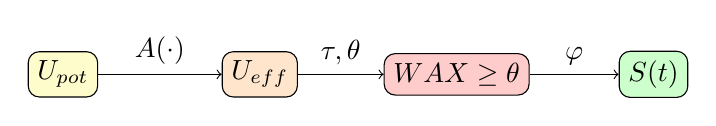
\begin{tikzpicture}[node distance=2.5cm, auto]
    \node (upot) [draw, rounded corners, fill=yellow!20] {$U_{pot}$};
    \node (ueff) [draw, rounded corners, fill=orange!20, right of=upot] {$U_{eff}$};
    \node (wax) [draw, rounded corners, fill=red!20, right of=ueff] {$WAX \geq \theta$};
    \node (st) [draw, rounded corners, fill=green!20, right of=wax] {$S(t)$};

    \draw[->] (upot) -- node[above] {$A(\cdot)$} (ueff);
    \draw[->] (ueff) -- node[above] {$\tau, \theta$} (wax);
    \draw[->] (wax) -- node[above] {$\varphi$} (st);
\end{tikzpicture}
\end{center}

\vspace{0.5em}
\begin{tabular}{|c|l|l|}
\hline
\textbf{Stage} & \textbf{Meaning} & \textbf{Chapter} \\
\hline
$U_{pot}$ & Potential utility (if fully aware) & Ch. 10 \\
$U_{eff}$ & Effective utility (awareness-weighted) & Ch. 11 \\
$WAX \geq \theta$ & Willingness exceeds action threshold & Ch. 12 \\
$S(t)$ & Sustained behavioral state over time & Ch. 13 \\
\hline
\end{tabular}
\end{tcolorbox}

\textbf{Interpretation:} Not all potential value translates to effective value (awareness gap). Not all effective value triggers action (willingness threshold). Not all actions sustain (journey dynamics).


% =============================================================================
% SECTION 8: CHAPTER INTEGRATION MATRIX
% =============================================================================
\section{Chapter Integration Matrix}
\label{sec:25-integration}

Each chapter contributes specific components to the Master Problem:

\begin{tcolorbox}[colback=gray!5!white,colframe=gray!75!black,
    title=\textbf{Chapter Contribution Matrix (Selected)}]
\small
\begin{tabular}{|c|l|l|}
\hline
\textbf{Ch.} & \textbf{Title} & \textbf{Contribution to MP-1} \\
\hline
1 & Introduction & Problem framing \\
5 & Complementarity & $\gamma$ matrix structure \\
9 & Context & $\Psi$ dynamics, endogeneity \\
10 & FEPSDE & Utility dimensions $d$ \\
11 & Awareness & $A(\cdot)$ function \\
12 & Willingness & WAX formula, $\theta$ threshold \\
13 & BCJ & Phase $\varphi$, journey dynamics \\
16 & $P_{eff}$ & Objective function \\
17-19 & Interventions & $\vec{I}$ design, phase/segment \\
20 & Portfolios & C1--C7 constraints, K* \\
\hline
\end{tabular}
\end{tcolorbox}

\textbf{Completeness:} The full mapping (140 axioms, 62 theorems) is in Appendix MP.


% =============================================================================
% SUMMARY
% =============================================================================
\section{Summary}
\label{sec:25-summary}

This chapter presented the complete optimization problem that unifies the EBF framework:

\begin{enumerate}
    \item \textbf{Master Problem:} $\max \sum_t \delta^t P_{eff}(S_t, I_t, \Psi_t)$
    \item \textbf{10C State Space:} Complete representation of behavioral state
    \item \textbf{Constraints C1--C7:} Operational bounds on intervention design
    \item \textbf{Dynamics:} Bellman equation with endogenous context
    \item \textbf{Properties:} Non-concavity, multiple equilibria, K vs Q
    \item \textbf{4-Stage Pipeline:} $U_{pot} \to U_{eff} \to WAX \to S(t)$
\end{enumerate}

\textbf{The Key Insight:} The optimization problem IS the framework. Understanding MP-1 is understanding EBF.


% =============================================================================
% PRACTICAL WORKFLOW
% =============================================================================
\section{Practical Workflow: From Problem to Portfolio}
\label{sec:25-workflow}

The Master Problem provides the theory---this section provides the practice. Follow these steps to apply EBF systematically.

\subsection{The 7-Step EBF Workflow}
\label{sec:25-7step}

\begin{tcolorbox}[colback=blue!5!white,colframe=blue!75!black,
    title=\textbf{7-Step Workflow: Context $\to$ Model $\to$ Portfolio $\to$ Learn}]

\textbf{Phase A: CONTEXT (Step 1) --- The Foundation}

\textbf{Step 1: Define Context ($\Psi$)}
\begin{itemize}[noitemsep]
    \item \textbf{Physical:} Where does the behavior occur? (Home, workplace, store, online)
    \item \textbf{Social:} Who else is present? (Alone, peers, authority, strangers)
    \item \textbf{Temporal:} When? (Morning/evening, deadline proximity, life stage)
    \item \textbf{Institutional:} What rules apply? (Regulations, norms, defaults)
    \item \textbf{Cognitive:} What mental state? (Stressed, depleted, distracted)
    \item \textit{Why first?} Context determines which parameters apply, which interventions work, and how segments respond
    \item \textit{Tool:} Context Checklist (see Appendix V)
\end{itemize}

\vspace{1em}
\textbf{Phase B: UNDERSTAND (Steps 2--3)}

\textbf{Step 2: Define Behavioral Problem (within Context)}
\begin{itemize}[noitemsep]
    \item What behavior should change? (Target behavior)
    \item Who is the target population? (Segment)
    \item What is the current baseline? (Status quo)
    \item How does context $\Psi$ shape the problem?
    \item \textit{Tool:} Free-form analysis, domain expertise
\end{itemize}

\textbf{Step 3: Search Similar Cases (Context-Filtered)}
\begin{itemize}[noitemsep]
    \item Query Case Registry for similar interventions \textit{in similar contexts}
    \item Extract prior effect sizes and context factors
    \item Identify what worked (and what didn't) \textit{under which $\Psi$}
    \item \textit{Tool:} \texttt{/case --domain <X> --context <Y>}
\end{itemize}

\vspace{1em}
\textbf{Phase C: MODEL (Step 4)}

\textbf{Step 4: Map to 10C State Space}
\begin{itemize}[noitemsep]
    \item WHO: Which welfare levels? ($L$)
    \item WHAT: Which utility dimensions? ($d$ in FEPSDE)
    \item HOW: What complementarities? ($\gamma$)
    \item WHEN: Context factors from Step 1 ($\Psi$) $\leftarrow$ \textit{already defined!}
    \item WHERE: Which parameters apply for this $\Psi$? ($\Theta$)
    \item AWARE: Current awareness? ($A$)
    \item READY: Current willingness? ($W$)
    \item STAGE: Journey phase? ($\varphi$)
    \item \textit{Tool:} \texttt{/design-model --mode schnell}
\end{itemize}

\vspace{1em}
\textbf{Phase D: DESIGN (Steps 5--6)}

\textbf{Step 5: Design Intervention(s)}
\begin{itemize}[noitemsep]
    \item Select 10C target dimension(s) to change
    \item Choose intervention type (AWARE$\uparrow$, WHEN$\to$, WHAT$\uparrow$, etc.)
    \item Check Phase-Dimension Affinity ($\alpha > 0.5$?)
    \item Check Segment Multiplier \textit{for this context} ($\sigma > 0$?)
    \item \textit{Tool:} \texttt{/design-intervention --mode standard}
\end{itemize}

\textbf{Step 6: Assemble Portfolio}
\begin{itemize}[noitemsep]
    \item Check Crowding-Out (C2): $\gamma(I_i, I_j) \geq \gamma_{min}$?
    \item Check Budget (C1): $\sum c_j \cdot I_j \leq B$?
    \item Check Portfolio Size (C7): $K \leq K^*(\Psi)$ $\leftarrow$ \textit{context-dependent!}
    \item Apply remaining constraints C3--C6
    \item \textit{Decision:} Start with $K=3$, add only if marginal benefit exceeds crowding cost
\end{itemize}

\vspace{1em}
\textbf{Phase E: PREDICT \& LEARN (Step 7)}

\textbf{Step 7: Predict, Implement, Close Loop}
\begin{itemize}[noitemsep]
    \item Calculate expected $P_{eff}$ using context-calibrated parameters
    \item Document prediction with confidence interval
    \item Register in Intervention Registry: \texttt{/intervention-manage new}
    \item After implementation: Record actual outcomes
    \item Compare prediction vs. result (Deviation Analysis)
    \item \textbf{Key Question:} Was deviation due to wrong $\Psi$ characterization?
    \item Update parameters and Case Registry: \texttt{/intervention-manage close}
\end{itemize}

\end{tcolorbox}

\begin{tcolorbox}[colback=green!5!white,colframe=green!75!black,
    title=\textbf{Why Context First?}]
\small
Context ($\Psi$) is the \textbf{master moderator} of behavioral interventions:

\begin{enumerate}[noitemsep]
    \item \textbf{Parameters depend on context:} Loss aversion $\lambda$ differs at home vs. workplace
    \item \textbf{Interventions work differently:} Social norms effective with peers, not alone
    \item \textbf{Segments respond differently:} Same person behaves differently under stress
    \item \textbf{Crowding-out is context-specific:} Financial incentives crowd out intrinsic motivation more in social contexts
\end{enumerate}

\textit{``Same intervention, different context, different outcome''} --- This is why Step 1 defines $\Psi$ before anything else.
\end{tcolorbox}

\subsection{Workflow Decision Tree}
\label{sec:25-decision-tree}

\begin{tcolorbox}[colback=yellow!5!white,colframe=yellow!75!black,
    title=\textbf{Entry Point Selection: Where Do I Start?}]

\textbf{Golden Rule:} \textit{Always start with context (Step 1).} Even if you think you know the problem, explicitly characterizing $\Psi$ prevents costly mistakes later.

\textbf{If you have:}
\begin{itemize}[noitemsep]
    \item A specific behavioral problem $\to$ Step 1 (Context) $\to$ Step 2 (Problem)
    \item An existing intervention to evaluate $\to$ Step 1 (Context) $\to$ Step 5 (backward validation)
    \item A new domain to explore $\to$ Step 1 (Context) $\to$ Step 3 (\texttt{/case})
    \item Parameter uncertainty $\to$ Step 1 (Context) $\to$ LLMMC (Appendix AN)
    \item A running project to close $\to$ Go directly to Step 7
\end{itemize}

\textbf{If you're unsure:}
\begin{enumerate}[noitemsep]
    \item \textbf{First:} Characterize context ($\Psi$) using the 5-dimension checklist
    \item Run \texttt{/case --domain <X> --context <Y>} to see what's been done in similar contexts
    \item Run \texttt{/design-model --mode schnell} to get a 10C model in 10 minutes
    \item Iterate from there
\end{enumerate}

\end{tcolorbox}

\subsection{Constraint Checklist}
\label{sec:25-constraint-checklist}

Before finalizing any portfolio, verify all constraints:

\begin{tcolorbox}[colback=red!5!white,colframe=red!75!black,
    title=\textbf{Portfolio Validation Checklist (C1--C7)}]
\small
\begin{tabular}{|c|l|l|c|}
\hline
\textbf{C} & \textbf{Constraint} & \textbf{Check} & $\checkmark$ \\
\hline
C1 & Budget & $\sum c_j \cdot I_j \leq B$ & $\square$ \\
C2 & Crowding-Out & No Social+Financial without justification & $\square$ \\
C2 & Crowding-Out & No Financial+Commitment without justification & $\square$ \\
C3 & Timing & Interventions match BCJ phase ($\alpha > 0.5$) & $\square$ \\
C4 & Capacity & Implementation capacity available & $\square$ \\
C5 & Ethics & Autonomy preserved, informed consent & $\square$ \\
C6 & Segment & Segment multiplier $\sigma > 0$ (no backfire) & $\square$ \\
C7 & Portfolio Size & $K \leq K^*$ (typically 3--7) & $\square$ \\
\hline
\end{tabular}
\end{tcolorbox}

\subsection{Tool Reference}
\label{sec:25-tools}

Quick reference for EBF skills:

\begin{center}
\begin{tabular}{|l|l|l|}
\hline
\textbf{Task} & \textbf{Skill} & \textbf{Workflow Step} \\
\hline
Define context & Context Checklist (Appendix V) & Step 1 \\
Find similar cases & \texttt{/case --context <X>} & Step 3 \\
Design 10C model & \texttt{/design-model} & Step 4 \\
Design intervention & \texttt{/design-intervention} & Step 5 \\
Register \& predict & \texttt{/intervention-manage new} & Step 7 \\
Close \& learn & \texttt{/intervention-manage close} & Step 7 \\
Add new case & \texttt{/case-manage add} & Step 7 \\
\hline
\end{tabular}
\end{center}


% =============================================================================
% WHAT COMES NEXT
% =============================================================================
\section{What Comes Next}
\label{sec:25-next}

With the complete optimization problem and practical workflow defined, practitioners can:

\begin{enumerate}
    \item \textbf{Apply the 7-Step Workflow:} Use the structured approach above for any behavioral intervention project
    \item \textbf{Calibrate parameters:} Use Appendix BBB and empirical data to estimate $\Theta$
    \item \textbf{Solve computationally:} Use Appendix AN (LLMMC) for parameter estimation under uncertainty
    \item \textbf{Validate predictions:} Test EBF predictions against observed behavioral outcomes
    \item \textbf{Close the loop:} Update parameters and Case Registry with learnings
\end{enumerate}

The framework is now complete---ready for application, calibration, and empirical testing.


% =============================================================================
% READING PATH BOX
% =============================================================================
\begin{tcolorbox}[colback=blue!5!white,colframe=blue!75!black,
    title=\textbf{Reading Path}]
\textbf{Prerequisites:} Chapters 1--24 (or selective reading via Chapter Matrix)

\textbf{This Chapter:} The Complete Optimization Problem

\textbf{Next:}
\begin{itemize}[noitemsep]
    \item For formal details: Appendix MP (CORE-MASTER)
    \item For solution methods: Appendix AN (METHOD-LLMMC)
    \item For parameter calibration: Appendix BBB (CORE-WHERE)
    \item For applications: DOMAIN Appendices (AA--AG)
\end{itemize}
\end{tcolorbox}


\end{chapter}
